\section{Merging of models}
From the previous section three linearized expressions can be extracted. These are ow to be combinded such that a final expression is derived, representing the entire system.
The expressions are as follows:

\begin{align}
\tau_a(s)&=\frac{K_t}{R_A}- \Theta_m(s)\cdot(s^2\cdot J_T+s(\frac{k_t+k_e}{R_a}+B_T))\label{eq:1}\\
\Theta_m(s)&= \frac{(J_p+m_p\cdot l^2)s^2\cdot \Theta_p(s)}{m_p\cdot l \cdot r_w \cdot N_{ms}\cdot N_{sw}}-\frac{g\cdot \Theta_p(s)}{s^2 \cdot r_w\cdot N_{ms}\cdot N_{sw}} \label{eq:2}\\
2\cdot F_F(\Theta_p(s))&=\Theta_p(s)(s^2(J_p+m_p\cdot l^2)(m_p+m_c)-m_p^2\cdot l^2)-(m_p^2 + m_c)l\cdot g \label{eq:3}
\end{align}

Combining \author{eq:1} and \autoref{eq:2} yields:
\begin{equation}
F_F(\Theta_p(s))=\frac{\frac{k_t}{R_a}\cdot V_a-(\frac{(J_p+m_p\cdot l^2)\Theta_p(s)}{m_p\cdot l\cdot r_w \cdot N_{ms}\cdot N_{sw}}-\frac{g\cdot \Theta_p(s)}{s^2\cdot r_w \cdot N_{ms}\cdot N_{sw}})(s^2\cdot J_t+s(\frac{k_t\cdot k_e}{R_a}+B_T))}{r_w} \label{eq:4}
\end{equation}
Note that the applied force $F_F(\Theta_p(s))$ is eual to the torque $\tau_a(s)$ when multiplied with the wheel ratio $r_w$, as torque is the product of force and length. \newpar
Now the motor model is combined  with the link-expression. This allows to connect all three equations. This is done by inserting \autoref{eq:4} into \autoref{eq:3}.
\begin{align}
(\Theta_p(s)(s^2(J_p+m_p\cdot l^2)(m_p+m_c)-&m_p^2\cdot l^2)-(m_p^2 + m_c)l\cdot g )\cdot r_w  \\ \nonumber
=\frac{k_t}{R_a}\cdot V_a-(\frac{(J_p+m_p\cdot l^2)\Theta_p(s)}{m_p\cdot l\cdot r_w \cdot N_{ms}\cdot N_{sw}}-&\frac{g\cdot \Theta_p(s)}{s^2\cdot r_w \cdot N_{ms}\cdot N_{sw}})(s^2\cdot J_t+s(\frac{k_t\cdot k_e}{R_a}+B_T))
\end{align}

The deriviation of the transferfunction of the entire system is in the appendix \todo{ref}. The final expression is fairly large, why each term has been given a letter to represent it in the transfer function here.
\begin{equation}
\frac{\Theta_p}{V_a}=\frac{k_t\cdot s}{R_a(s^3\cdot A + s^2 \cdot B + s(C_D)-E)}
\end{equation}






The linear model for the motors and wheels system and the one for the inverted pendulum, are in this section merged to form the linear model for the segway. The linear model for the inverted pendulum is shown in \autoref{eq:invPenLin_Merge}, and the linear model for the motors and wheels are shown in \autoref{eq:motorWheel_Merge}.

\begin{equation}
\frac{F_F(s)}{V_a(s)} = \frac{0.049s}{0.040s + 1}
\label{eq:motorWheel_Merge}
\end{equation}

\begin{align}
\frac{\theta_p(s)}{F_F(s)}=\frac{\frac{1}{l\cdot m_c}}{s^2-\frac{g\cdot (m_p+m_c)}{l\cdot m_c}}=\frac{2.377}{s^2 - 37.369}
\label{eq:invPenLin_Merge}
\end{align}

To merge these transfer functions, with the purpose of achieving one transfer function with $V_a(s)$ as input and $\theta_p(s)$ as output. The two transfer functions, \autoref{eq:invPenLin_Merge} and \autoref{eq:motorWheel_Merge}, are multiplied, since the two transfer functions are in series as shown in \autoref{fig:modelOverall} and can therefore be multiplied to get the output. This yields the transfer function for the segway shown in \autoref{eq:segwayTf}.

\begin{align}
\frac{\theta_p(s)}{V_a(s)} &= \frac{2.9s}{s^3 + 25s^2 - 37.5s - 943.75} = \frac{2.9s}{(s + 25)(s + 6.15)(s - 6.14)}
\label{eq:segwayTf}
\end{align} 
Now that the combined transfer function has been determined, it needs to be verified through comparison with test results.

It is decided to remove the pole in -25, based on the impulse response, as it is seen that this pole does not have much influence. Thus, the system is reduced to a 2'nd order system, with a zero in zero.

This is put into matlab to do parameter estimation again.
We see that the gain is off by a factor of about 3 by looking at the input/output graphs of the measurements, so the gain is changed. This is thus the model we use as our guess for Matlab to estimate from.
\begin{figure}[H]
    \centering
    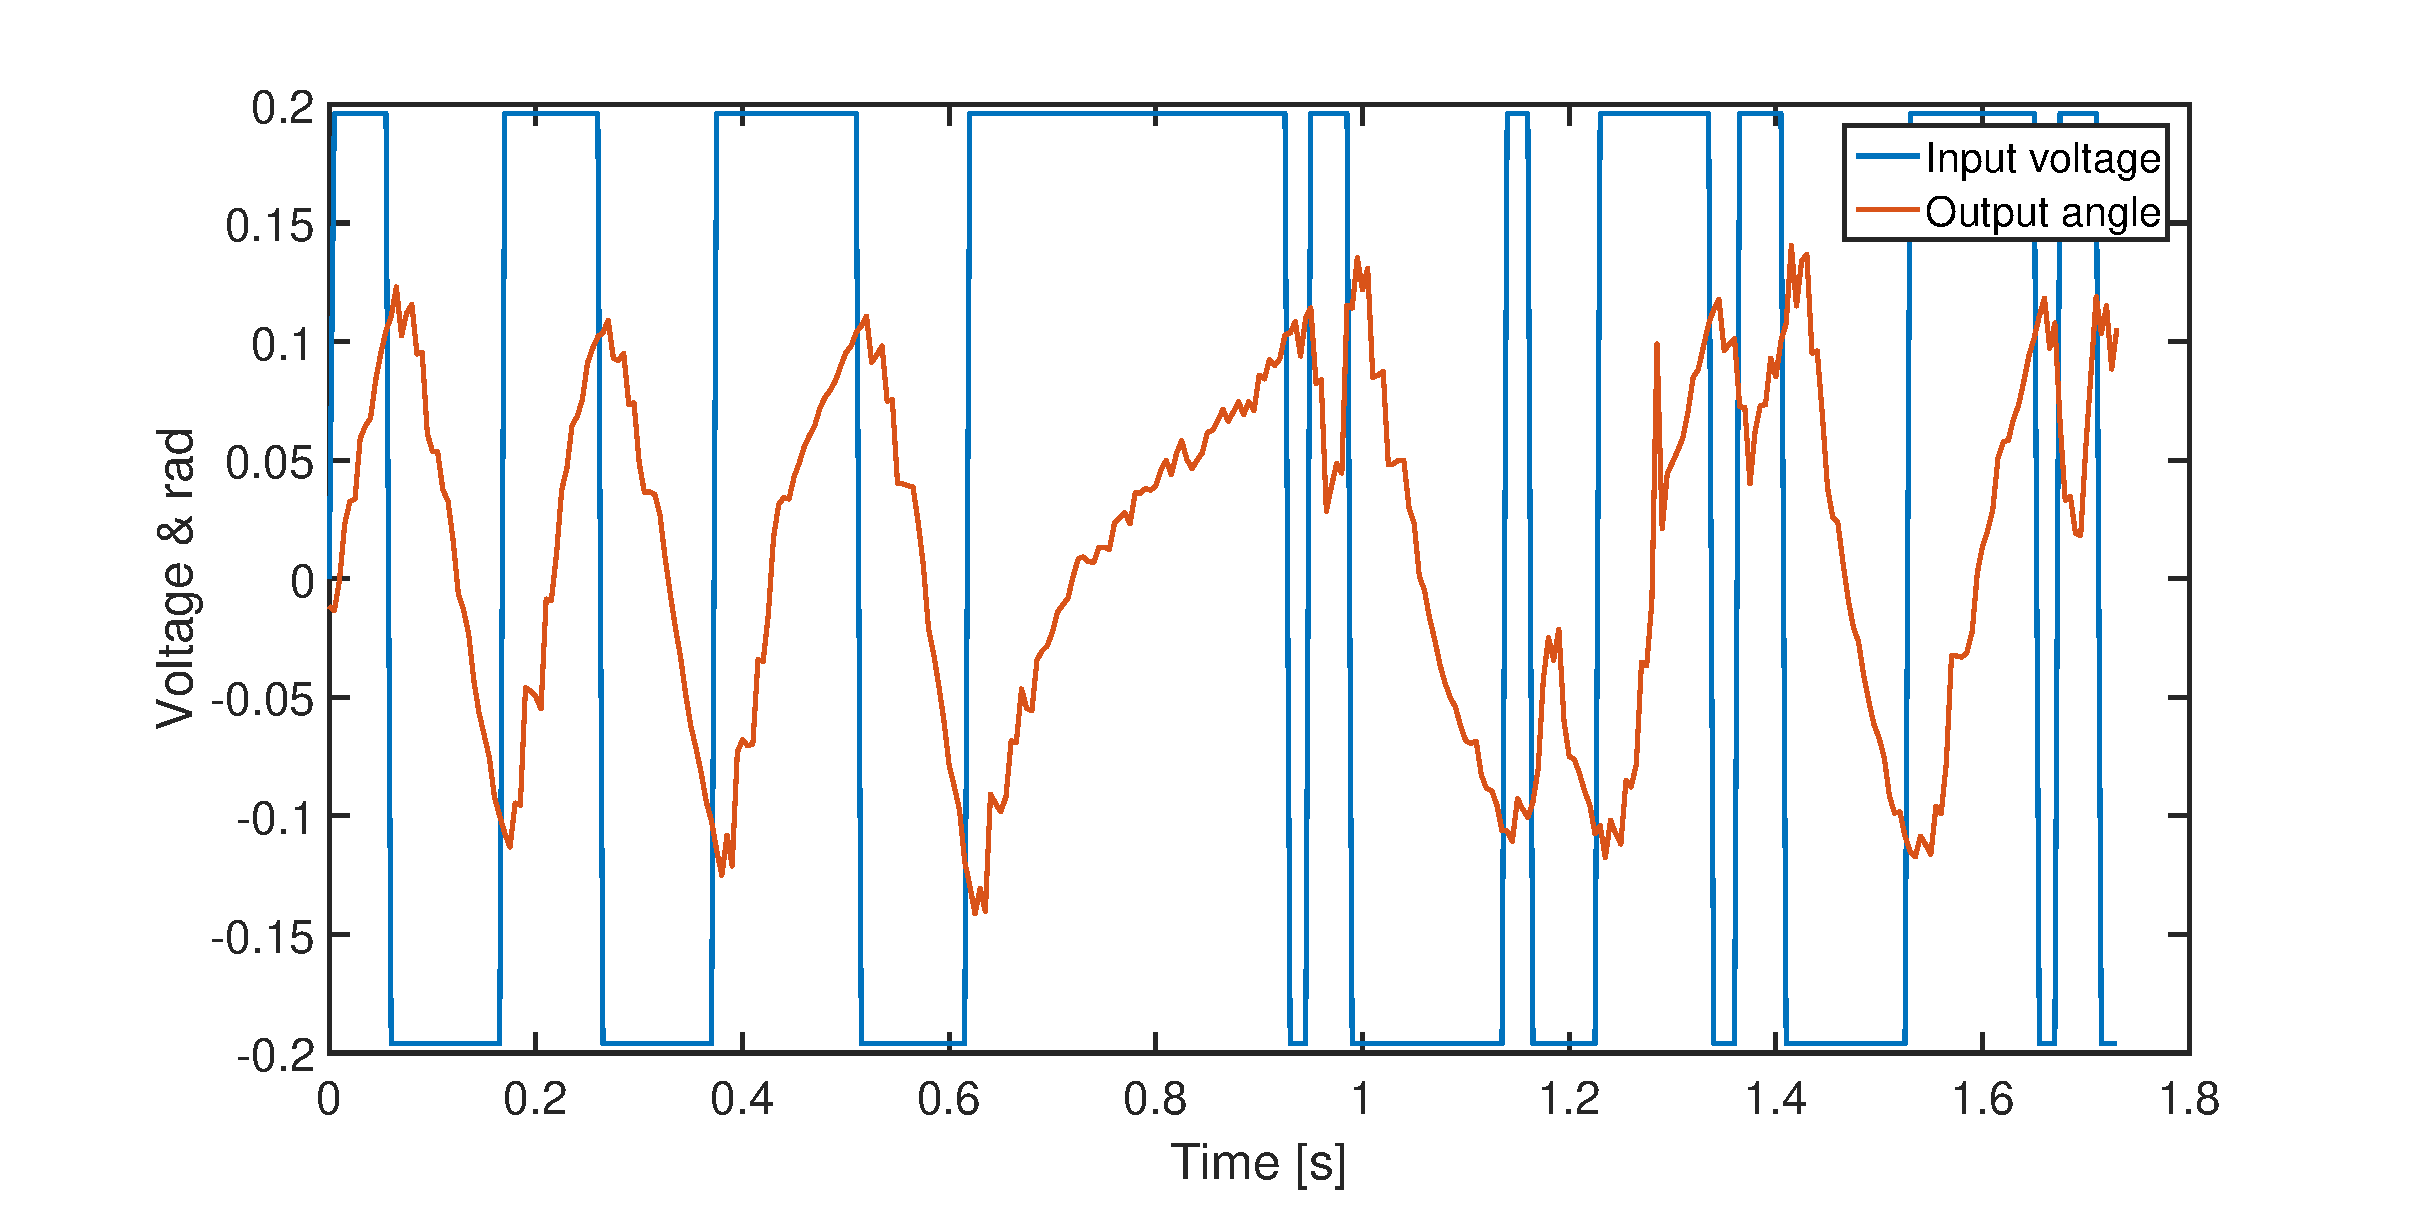
\includegraphics[width = \textwidth]{ParameterEstimationSegway.eps}
    \caption{Input voltage and output angle of segway for model verification.}
    \label{fig:paramEst3}
\end{figure} 


\begin{figure}[H]
    \centering
    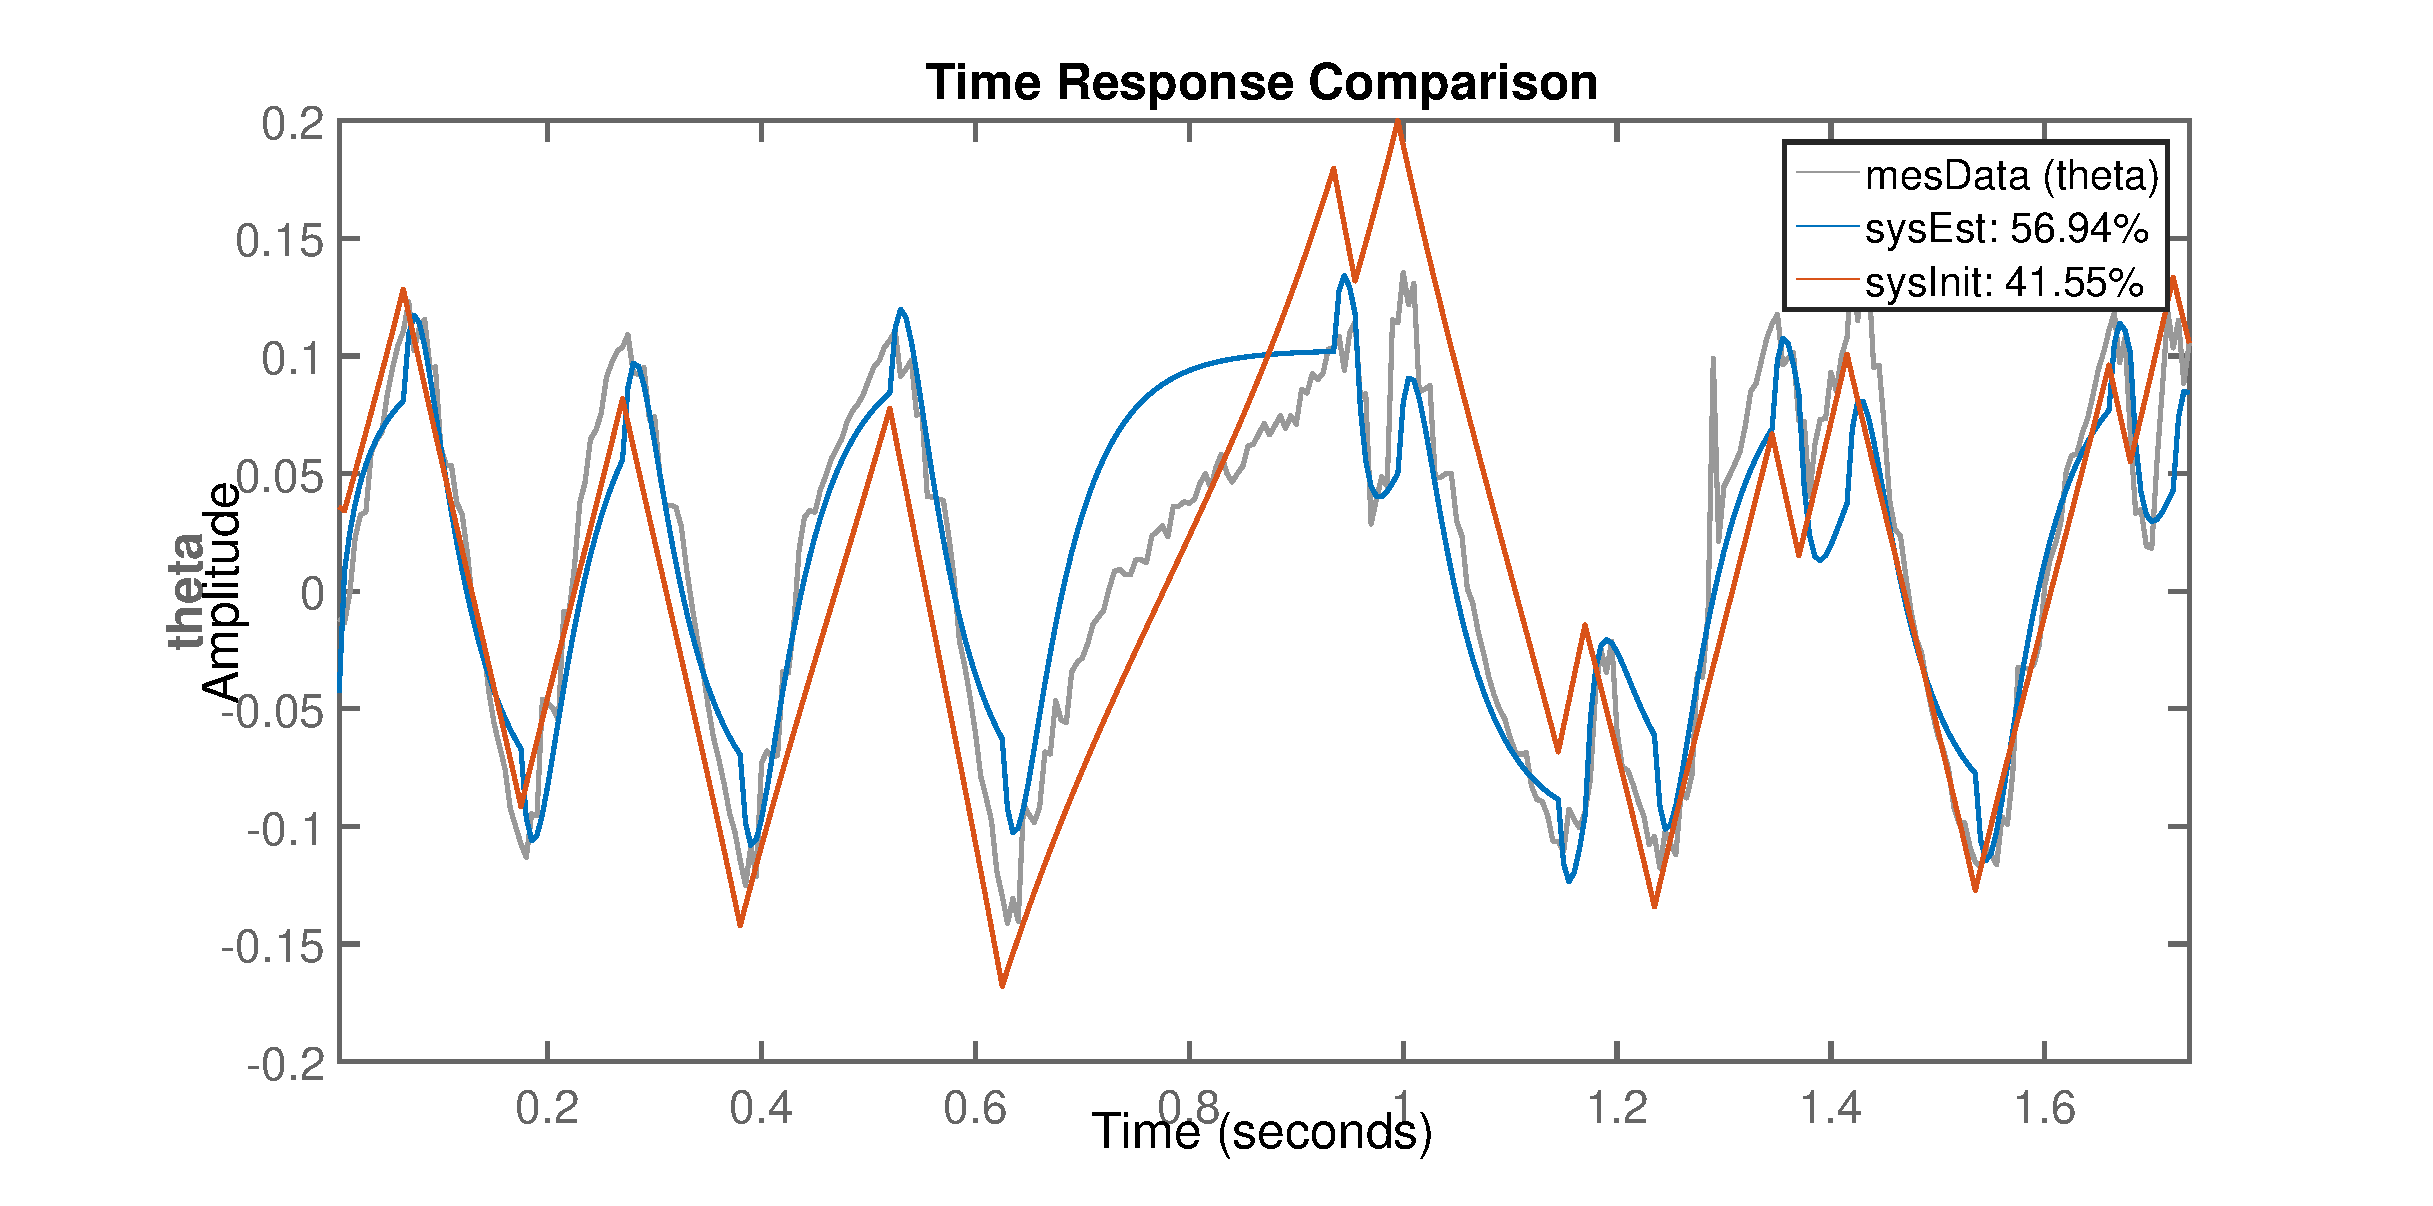
\includegraphics[width = \textwidth]{ParameterEstimationSegway2.eps}
    \caption{System initial guess, measurements and Matlab estimate.}
    \label{fig:paramEst4}
\end{figure} 

Matlab provides the following transfer function:

\begin{align}
\frac{\theta_p(s)}{V_a(s)} &= \frac{-2.015 s + 100.2}{s^2 + 112.3 s + 1918} = \frac{-2.015 (s - 49.7)}{(s + 91)(s + 21)}
\label{eq:wrongTF}
\end{align} 

